\chapter{Appendices}\label{sec:appendices}

\section{Appendix A: Mathematical Notation}\label{sec:appendix-a-mathematical-notation}

{\def\LTcaptype{table} % do not increment counter
\begin{longtable}[]{@{}ll@{}}
\toprule\noalign{}
Symbol & Description \\
\midrule\noalign{}
\endhead
\bottomrule\noalign{}
\endlastfoot
\(b\) & Binary bit (\(\in \{0, 1\}\)) \\
\(x\) & Modulated BPSK symbol (\(\in \{-1, +1\}\)) \\
\(y\) & Received signal \\
\(n\) & Noise sample \\
\(h\) & Fading coefficient \\
\(\sigma^2\) & Noise variance \\
\(\text{SNR}\) & Signal-to-Noise Ratio (linear) \\
\(G\) & AF amplification gain \\
\(\mathbf{H}\) & MIMO channel matrix (\(\in \mathbb{C}^{2 \times 2}\)) \\
\(\mathbf{W}\) & Neural network weight matrix \\
\(\mathbf{b}\) & Bias vector \\
\(P_e\) & Bit error rate \\
\(Q(\cdot)\) & Gaussian Q-function \\
\(K\) & Rician K-factor \\
\(\beta\) & VAE KL weight \\
\(\lambda\) & Regularization parameter \\
\(\eta\) & Learning rate \\
\(\Delta\) & State space discretization step \\
\(\mathbf{A}, \mathbf{B}, \mathbf{C}, D\) & State space model matrices \\
\end{longtable}
}

\section{Appendix B: Model Architectures and Hyperparameters}\label{sec:appendix-b-model-architectures-and-hyperparameters}

% column helpers
\newcolumntype{L}[1]{>{\raggedright\arraybackslash}p{#1}}
\newcolumntype{Y}{>{\raggedright\arraybackslash}X}

\begin{table}[ht]
\centering
\footnotesize
\setlength{\tabcolsep}{4pt}
\renewcommand{\arraystretch}{1.15}

\begin{tabularx}{\textwidth}{|L{2.1cm}|Y|L{3.2cm}|L{1.7cm}|L{2.3cm}|}
\hline
\textbf{Relay} &
\textbf{Network Topology} &
\textbf{Train Loss (LR)} &
\textbf{Total Params} &
\textbf{Implementation} \\
\hline
MLP (Minimal) &
Feedforward MLP, 5-symbol sliding window &
MSE, lr=0.01, 100 epochs &
169 &
NumPy (CPU) \\
\hline
Hybrid &
MLP + DF switching via learned SNR threshold ($\sim$5 dB) &
MSE (MLP only), lr=0.01 &
169 &
NumPy (CPU) \\
\hline
VAE &
Encoder--decoder latent model (7$\to$8$\to$1) &
$\beta$-VAE ($\beta=0.1$), Adam lr=$10^{-3}$ &
1{,}777 &
PyTorch (CUDA) \\
\hline
CGAN (WGAN-GP) &
Conditional GAN (generator + critic) &
WGAN-GP, Adam lr=$10^{-4}$ &
2{,}946 &
PyTorch (CUDA) \\
\hline
Transformer &
2-layer encoder, 4 heads, $d_{\text{model}}=32$ &
MSE, Adam lr=$10^{-3}$ &
17{,}697 &
PyTorch (CUDA/CPU) \\
\hline
Mamba S6 &
Selective SSM, 2 S6 layers &
MSE, Adam lr=$10^{-3}$ &
24{,}001 &
PyTorch (CUDA/CPU) \\
\hline
Mamba2 (SSD) &
Selective SSM with SSD kernel (2 layers) &
MSE, Adam lr=$10^{-3}$, clip=1.0 &
26{,}179 &
PyTorch (CUDA) \\
\hline
\end{tabularx}

\caption{Comparison of relay models, training objectives, parameter counts, and implementations.}
\label{tab:relay_comparison}
\end{table}

\section{Appendix C: Software Architecture}\label{sec:appendix-c-software-architecture}

\noindent
All numerical results reported in chapter \ref{sec:experiments} were generated using the framework shown in figure \ref{fig:relaynet_uml}, ensuring consistent evaluation across classical and learning-based relay architectures.The project is implemented as a modular Python package (\texttt{relaynet}).
The framework uses object-oriented design with a common \texttt{Relay} base class, enabling polymorphic relay swapping. Monte Carlo simulation is implemented in \texttt{runner.py} with configurable trial count, bit count, and SNR range. All MIMO operations use vectorized PyTorch for GPU acceleration.

\subsection{Testing} 126 automated tests (pytest) cover all channels, modulation (BPSK, QPSK, 16-QAM, 16-PSK), relay strategies, simulation, statistics, and modulation-comparison modules with 100\% pass rate.

\subsection{Reproducibility} Random seeds are controlled at the source (bit generation) and noise (per-trial seeding) levels to ensure reproducible results.
\begin{figure}[bt]
\centering
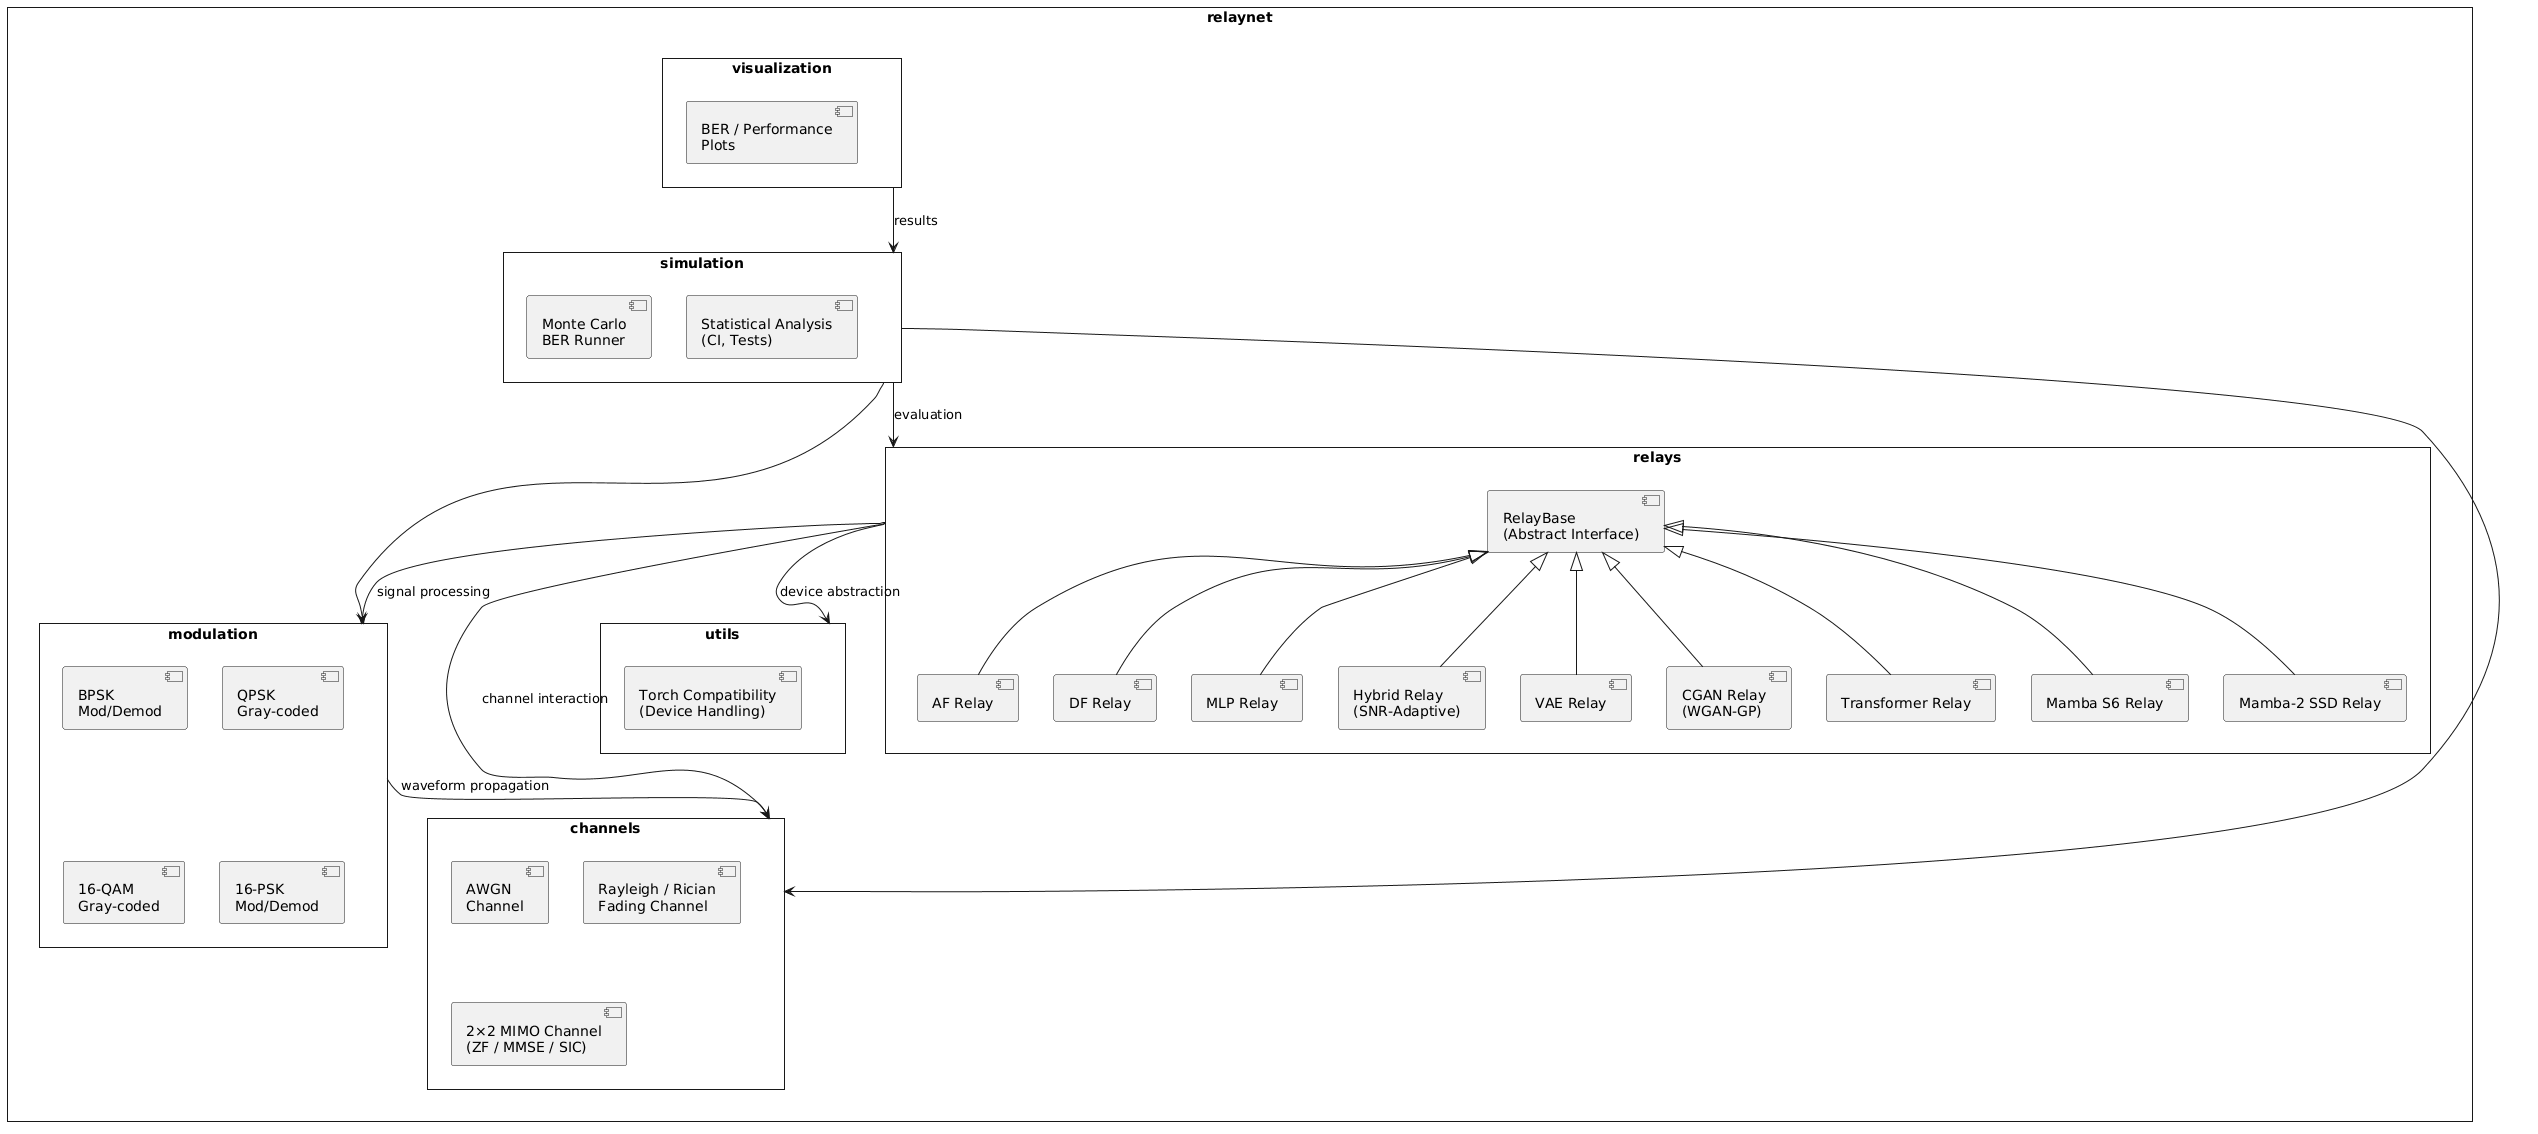
\includegraphics[width=\textwidth,angle=-90,scale=1.5]{results/relaynet_sw_architecture.png}
\caption{UML-style component diagram of the \texttt{relaynet} simulation framework.}
\label{fig:relaynet_uml}
\end{figure}



\clearpage

\section{Appendix D: Normalized 3K-Parameter Configurations}\label{sec:appendix-d-normalized-3k-parameter-configurations}

{\def\LTcaptype{table} % do not increment counter
\begin{longtable}[]{@{}
  >{\raggedright\arraybackslash}p{(\linewidth - 6\tabcolsep) * \real{0.2500}}
  >{\raggedright\arraybackslash}p{(\linewidth - 6\tabcolsep) * \real{0.2500}}
  >{\raggedright\arraybackslash}p{(\linewidth - 6\tabcolsep) * \real{0.2500}}
  >{\raggedright\arraybackslash}p{(\linewidth - 6\tabcolsep) * \real{0.2500}}@{}}
\toprule\noalign{}
\begin{minipage}[b]{\linewidth}\raggedright
Model
\end{minipage} & \begin{minipage}[b]{\linewidth}\raggedright
Parameters
\end{minipage} & \begin{minipage}[b]{\linewidth}\raggedright
Window
\end{minipage} & \begin{minipage}[b]{\linewidth}\raggedright
Hidden / Architecture
\end{minipage} \\
\midrule\noalign{}
\endhead
\bottomrule\noalign{}
\endlastfoot
MLP-3K & 3,004 & 11 & hidden=231 \\
Hybrid-3K & 3,004 & 11 & hidden=231 (+ DF switch) \\
VAE-3K & 3,037 & 11 & latent=10, hidden=(44, 20) \\
CGAN-3K & 3,004 & 11 & noise=8, g\_hidden=(30, 30, 16), c\_hidden=(32, 16) \\
Transformer-3K & 3,007 & 11 & d\_model=18, heads=2, layers=1 \\
Mamba-3K & 3,027 & 11 & d\_model=16, d\_state=6, layers=1 \\
Mamba2-3K & 3,004 & 11 & d\_model=15, d\_state=6, chunk\_size=8, layers=1 \\
\end{longtable}
}

All 3K configurations use a window size of 11 (vs.~5 for original MLP/Hybrid, and 11 for original sequence models) to provide a common input context. The parameter counts are within ±1.2\% of the 3,000 target.

\begin{center}\rule{0.5\linewidth}{0.5pt}\end{center}

%% ── Hebrew Abstract (Back Matter) ───────────────────────────
